\documentclass[10pt, conference]{IEEEtran}
\usepackage[english]{babel}
\usepackage[usenames]{color}
\usepackage{colortbl}
\usepackage{comment}
\usepackage{graphicx}
\usepackage{epsfig}
\usepackage{array, colortbl}
\usepackage{listings}
\usepackage{epstopdf}
\usepackage{multirow}
\usepackage{rotating}
%\usepackage{subfigure}
%\usepackage{subfig}
\usepackage{float}
\usepackage[obeyspaces,hyphens,spaces]{url}
\usepackage{balance}
\usepackage{fancybox}
\usepackage{scalefnt}
\usepackage[normalem]{ulem}
%\pagestyle{plain}
\pagenumbering{arabic}
\pagestyle{empty}
\clubpenalty = 10000
\widowpenalty = 10000
\displaywidowpenalty = 10000
\usepackage{cleveref}
\usepackage{latexsym}
\usepackage{amsfonts}
\usepackage{amssymb}

\usepackage{graphicx}
\usepackage{caption}
\usepackage{subcaption}


\newcommand*{\escape}[1]{\texttt{\textbackslash#1}}
\newcommand*{\escapeI}[1]{\texttt{\expandafter\string\csname #1\endcsname}}
\newcommand*{\escapeII}[1]{\texttt{\char`\\#1}}

\makeatletter
\renewcommand{\paragraph}[1]{\noindent\textsf{#1}.}


\title{Hadoop MapReduce on Amazon EC2}
\author{Zeinab Kermansaravi, Mohammed Sayagh
    \\
    \emph{zeinab.kermansaravi, mohammed.sayagh}@polymtl.ca}

\begin{document}
\maketitle

\begin{abstract}
When Yahoo, Google, Facebook, and other companies extended their services to web-scale, the amount of data they collected routinely from user interactions online have overwhelmed the capabilities of traditional IT architectures. Hadoop is an open source system which is used as the core platform for structuring Big data, and solves the problems of formatting it for subsequent analytic purposes. Hadoop uses a distributed computing architecture consisting of multiple servers using commodity hardware, making it relatively inexpensive to scale and support extremely large data stores. We set up the MapReduce framework to solve the problems in social networks and comparing Hadoop and Simple Linux Command performances, to show what can we do with Hadoop MapReduce, and when Hadoop is better than a simple Linux command line. We found that Linux command is efficient than Hadoop when the execution is on one machine (either standalone mode or pseudo distributed mode), however we found that Hadoop is efficient than command line when Hadoop is executed in many machines (five machines in our case) and specially when the data size is higher than around 29120 bytes.

\end{abstract}

\section{Introduction}
\label{sec:introduction}

\indent Today is the digital world in which by increasing digitization, the amount of structured and unstructured data being created and stored is exploding. The data is being generated from various sources such as transactions, social media, sensors, digital images, videos, audios and clickstreams for domains including healthcare, retail, energy and utilities. And also, to business and organizations, individuals contribute to the data volume. For instance, 30 billion content are being shared on Facebook every month; the photos viewed every 16 seconds in Picasa could cover a football field. \\
\indent Big Data is a relatively new phenomenon which increase the storage capacities, increase the processing power and able us to have more available data. Big Data analysis enables the executives to get the relevant data in less time for making decisions. Big data analytics is the process of examining large amounts of data of a variety of types to uncover hidden patterns, unknown correlations, and other useful information. Such information can provide competitive advantages over rival organizations and result in business benefits, such as more effective marketing and increased revenue. New methods of working with big data, such as Hadoop and MapReduce, offer alternatives to traditional data warehousing. 

\section{Background}

\indent Apache Hadoop is an open source software project that enables distributed processing of large data sets across clusters of commodity servers. It is designed to scale up from a single server to thousands of machines, with very high degree of fault tolerance. Rather than relying on high-end hardware, the resiliency of these clusters comes from the software's ability to detect and handle failures at the application layer. Hadoop changes the economics and the dynamics of large-scale computing which enables a computing solution that is scalable, cost effective, and flexible and fault tolerant.There are three modes to start a Hadoop cluster:\\
\indent 1- Local (Standalone) Mode\\
\indent 2- Pseudo-Distributed Mode\\
\indent 3- Fully-Distributed Mode\\

\indent Hadoop is composed of four core components, Hadoop Common, Hadoop Distributed File System (HDFS), MapReduce and Yet Another Resource Negotiator (YARN).
\begin{itemize}
\item Hadoop Common: which is a module containing the utilities that support the other Hadoop components.\\
\item Hadoop Distributed File System (HDFS): is a java-based file system that provides reliable data storage and access across all the nodes in a Hadoop cluster. It links together the file systems on many local nodes to create a single file system. HDFS is highly fault-tolerant and is designed to be deployed on low-cost hardware. HDFS provides high throughput access to application data and is suitable for applications that have large data sets. HDF can work under a variety of physical and systemic circumstances. By distributing storage and computation across many servers, the combined storage resource can grow with demand while remaining economical at every size.\\
\indent An HDFS cluster is comprised of a NameNode which manages the cluster metadata and DataNodes that store the data. Files and directories are represented on the NameNode by inodes. Inodes record attributes like permissions, modification and access times, or namespace and disk space quotas. The file content is split into large blocks (typically 128 megabytes), and each block of the file is independently replicated at multiple DataNodes. The blocks are stored on the local file system on the datanodes. The Namenode actively monitors the number of replicas of a block. When a replica of a block is lost due to a DataNode failure or disk failure, the NameNode creates another replica of the block. The NameNode maintains the namespace tree and the mapping of blocks to DataNodes, holding the entire namespace image in RAM. The NameNode does not directly send requests to DataNodes. It sends instructions to the DataNodes by replying to heartbeats sent by those DataNodes. The instructions include commands to: replicate blocks to other nodes, remove local block replicas, re-register and send an immediate block report, or shut down the node.\\
\item Map Reduce: is the heart of Hadoop which is a programming model used to process and generate vast amount of data (multi-terabyte data-sets) in parallel across a distributed cluster of processors or stand-alone computed. It was developed at Google for indexing Web pages and replaced their original indexing algorithms and heuristic in 2004. It is useful for large, long-running jobs that cannot be handled within the scope of a single request, tasks like: Analyzing application logs, aggregating related data from external sources, transforming data from one format to another, exporting data for external analysis, while it can also reduce network bandwidth, as the algorithm is passed around to where the data lives rather than transferring a potentially huge dataset to a client algorithm.\\
\indent The MapReduce framework has two functions to work, Map and Reduce which helps developers divide a query into steps. MapReduce job usually splits the input data-set into independent chunks which are processed by the map tasks in a completely parallel manner. The framework sorts the outputs of the maps, which are then input to the reduce tasks. Typically both the input and the output of the job are stored in a file-system. The framework takes care of scheduling tasks, monitoring them and re-executes the failed tasks.\\
\item and Yet Another Resource Negotiator (YARN): The next-generation MapReduce, which assigns CPU, memory and storage to applications running on a Hadoop cluster. It enables application frameworks other than MapReduce to run on Hadoop, opening up a wealth of possibilities.
\end{itemize}

MapReduce model cannot answer to all the problem, it has its limitations. Some recent works argues that MapReduce is much less sophisticated or efficient than parallel database query systems \cite{dewitt2008mapreduce}. Besides, MapReduce cannot be useful when the computation of a value depends on previously computed values. Also, if the data set is small, it is better to use a single reduce(map(data)) operation in single machine to compute. Another limitation is, while the index generated in the Map step is one dimensional, and the Reduce step must not generate a large amount of data or there will be a serious performance degradation. For example, CouchDB’s MapReduce may not be a good fit for full-text indexing or ad hoc searching. This is a problem better suited for a tool such as Lucene \cite{limit1}. Jignesh \cite{blanas2010comparison} also reveals the limitations of the MapReduce programming model for implementing joins.The MapReduce framework is increasingly being used to analyze large volumes of data. One important type of data analysis done with MapReduce is log processing, in which a click-stream or an evnt log is filtered, aggregated, or mined for patterns. As part of this analysis, the log often needs to be joined with reference data such as information about users. Although there have been many studies examining join algorithms in parallel and distributed DBMSs, the MapReduce framework is cumbersome for joins. MapReduce programmers often use simple but inefficient algorithms to perform joins.

The intrinsic limitation of MapReduce is, in fact, the “one-way scalability” of its design. Ziaiang Ma \cite{ma2010limitation} describes that the MapReduce design allows a program to scale up to process very large data sets, but constrains a program’s ability to process smaller data items. A significant amount of recent research work has addressed the problem of solving various data management problems in the cloud. The major algorithmic challenges in map-reduce computations involve balancing a multitude of factors such as the number of machines available for mappers/reducers, their memory requirements, and communication cost (total amount of data sent from mappers to reducers). Most past work provides custom solutions to specific problems, e.g., performing fuzzy joins in map-reduce, clustering, graph analyses, and so on. While some problems are amenable to very efficient map-reduce algorithms, some other problems do not lend themselves to a natural distribution, and have provable lower bounds. Clearly, the ease of "map-reducability" is closely related to whether the problem can be partitioned into independent pieces, which are distributed across mappers/reducers. What makes a problem distributable? Can we characterize general properties of problems that determine how easy or hard it is to find efficient map-reduce algorithms? This is a vision paper that attempts to answer the questions described above \cite{afrati2012vision}.



\section{Approach}
\label{sec:approach}
To conduct the experiments, we followed the instructions of the tutorial \cite{tutorial} to install Hadoop and run it in Pseudo distributed mode, and in order to execute Hadoop in Fully distributed mode, we followed the instructions of the tutorial \cite{tutorial2}.

We used five instances of type t2.micro to execute Hadoop in Fully distributed mode. 

To compute the number of words using the linux command, we used the following command : \textit{time cat file\_name | tr ' ' '\escape{n}' $|$ sort $|$ uniq -c}, where the file name can be changed by the character * to process all the files of a folder, which we use to experiment many files.

\section{Experiments}
\label{sec:experiments}

We conducted many experiments to evaluate the time difference between Hadoop execution in its three modes, and a simple Linux command line, and to evaluate what kind of problems that can be resolved by MapReduce. In this section we present the experiments that we did, we present for each one its approach, results, and discussion. 

\subsection{Experiment one and two}
The goal of the first and the second experiments consists of exploring the MapReduce examples, and comparing the execution time between Hadoop and Linux.
\subsubsection{Approach}
To do the two first experiments, we installed Hadoop by following the instructions of the tutorial \cite{tutorial} at first step, by executing Hadoop in pseudo distributed mode in the second step, and in fully distributed mode at the end. 
\subsubsection{Results}


\begin{center}
\begin{table}
\begin{center}
\begin{tabular}{|l|l|l|l|l|}
  \hline
 Execution environment & Mode & Time \\
  \hline
 Hadoop  & Pseudo-Distributed Mode & 0m7.701s \\
 Hadoop  & Fully-Distributed Mode & 0m6.852s \\
 Linux  & & 0m1.408s \\
  \hline
\end{tabular}

\caption{\label{ResultsExperiment1And2} Results of the first and second experiments}
\end{center}
\end{table}
\end{center}

Table \ref{ResultsExperiment1And2} highlights the results obtained by the first two experiments, we observe that the short time to compute the number of word occurrences in the book Ulyssess \cite{book0} is provided by the dedicated Linux command. 

\subsubsection{Discussion}
We found that Linux command line provide results faster than Hadoop plateform in the book Ulyssess, which can be explained by the size of the book which is not important. Hence, Linux command is better than Hadoop where the size of data is not important. 

Hadoop takes more time than simple Linux command, because it has to split data into many sections in the map phase, and has to collect the map results in the reduce phase, which can be harmful, and which makes the difference with the Linux command specially when data size is not important.

\subsection{Experiment three}
In the previous experiments, we found that Linux is better than Hadoop in the execution time and we referred this difference to the data size, in this experiment, we add more data to see when Hadoop gives results faster than Linux command line.
\subsubsection{Approach}
We conducted this experiment by increasing the data size and comparing execution time between Hadoop MapReduce and Linux command line.

Data used for this experiment consists of the books \cite{book0} \cite{book1} \cite{book2} \cite{book3} \cite{book4} \cite{book5} and 110 other files (the six books and the whole Wordpress forums archives \cite{WPArchives}). The total size of the whole data is 341880 bytes.

\subsubsection{Results}

\begin{figure}
	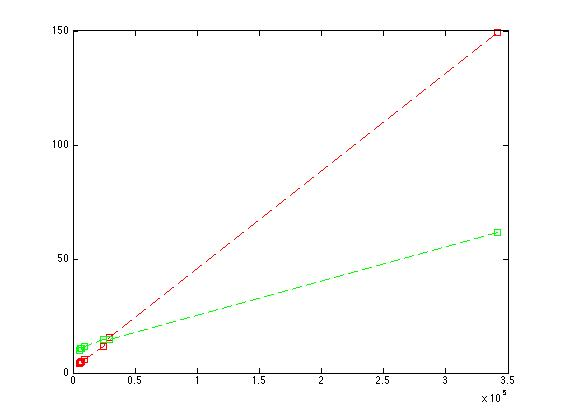
\includegraphics[width=0.5\textwidth]{plots/experiment3.jpg}
	\caption{\label{ResultExperiment3} WordCount execution time between Linux command and Hadoop Fully Distributed Mode (X-Axis : Data Size in byte, Y-Axis : Execution time in second) (Red line : Linux, Green line : WordCount MapReduce)}
\end{figure}

Figure \ref{ResultExperiment3} presents the difference between execution time provided by Hadoop MapReduce WordCount example, and by Command line. We found that Linux command line provides results in less time when data size is less than around 29120 bytes, whereas Hadoop provides results in less time than Linux command line when the size is higher than around 29120 bytes. 

We also found that Hadoop in Pseudo distributed mode provides results in 9.782s.

\subsubsection{Discussion}
We conclude that Hadoop is better than a simple command line when the size is important (more than 29120 bytes), and Linux is better than Hadoop if data size is not important. 


Dispatching data in different hosts (5 instances of type t2.micro in our case) could be consuming in term of time, however processing an important size of data in one host could be consuming too. Hence, we provide in this experience, the size that can be used to decide whenever we have to use Hadoop or only a simple Linux command. Moreover, while data size increases, Hadoop provides better results than Linux commands. 

Divide and conquer. Hadoop provides results in less time than Linux commands when data size is important, because it processes data in many hosts at the same time, however dispatching data has its price, which is related to the network performances. Hence, users should choose Hadoop if they are processing an important size of data, however they should choose Linux if they are processing a small data size.


\subsection{Experiment four}
In this experiment we modified the wordcount program, to compute only the occurrences containing the Word "Buck".
\subsubsection{Approach}


\begin{figure}
	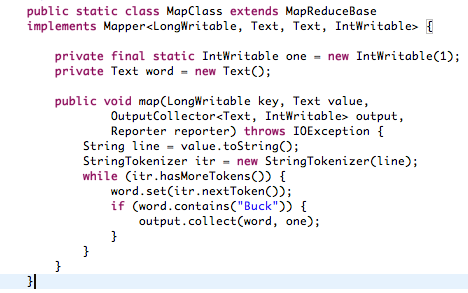
\includegraphics[width=0.5\textwidth]{plots/experiment4.png}
	\caption{\label{ResultExperiment4} Modified map method of the wordcount program.}
\end{figure}

We modified the map method of wordcount program, to filter the words mapped. Figure \ref{ResultExperiment4} highlights the modification provided to the wordcount program.

We also modified the linux command, by adding a pipeline that search only the words containing the word "Buck".

\subsubsection{Results}
The execution time of the modified program is 6.740s in pseudo distributed mode comparing to 9.782s for the wordcount program, and 6.736s in the fully distributed mode comparing to 9.743s for the wordcount program in the same execution mode. 

Linux provides the results of the same task in 2.598s comparing to 4.092s for wordcount. 

\subsubsection{Discussion}

The execution time of the modified mapreduce program in Hadoop is lower than the execution time of the wordcount example. This difference is because we filtered the words in the map step, hence the reduce task has less data because it reduces only the words containing the "Buck". Therefore, the time difference is due to the reduce tasks that are done in a smaller data comparing to the data reduced in a wordcount program.

Although we added new pipeline to the command line in order to get only the words containing "Buck", the execution time is slower than the command line computing the number of occurrences. We refer this difference principally to the fact that the first one print out only few lines comparing with the important number printed out in the second one.


\subsection{Problem}
In this section, we provide a solution to the problem "People you might know". It consists of proposing to each person his potential friends who are friends of his friends, sorted by people having a lot of mutual friends with him. For example if a person A knows a person B and C, where B is friend with D and E, and C is friend with D, therefore, we propose to A the person D and E.
\subsubsection{Approach}
We can use MapReduce to resolve such problem, because we can have simultaneous executions and reducing the results of each one (limits of MapReduce in Section \ref{sec:backgr-relat-work}).


The program contains two main steps, Map step and reduce step. In map step, we parse all the data file into a map, where the key is a person, and the value consists of each of his friends, for example if A is friend with B and C, we create two element in the map, which are (A,B) and (A,C). In the map step, we also add all the relations between a person friends, in the previous example, we add that B and C have a mutual friend who is A, and we get the key (B,C) and (C,B). To distinguish between the two first key and value and the second one, we add either the string "isFriend" or the string "isNotFriend". In the previous example, we got from the map step the following elements : (A; isFriend, B), (A; isFriend, C), (B; isNotFriend, C), and (C; isNotFriend, B).




\begin{center}
\begin{table}
\begin{center}
\begin{tabular}{|l|l|l|l|l|}
  \hline
 A & B,C \\
 B & A,D \\
 C & A,D \\
 D & B,C \\
  \hline
\end{tabular}

\caption{\label{ExampleProblem} Problem example  }
\end{center}
\end{table}
\end{center}

Lets take the example of Table \ref{ExampleProblem}. we will got the results of the Map step provided in Table \ref{MapExampleProblem}.




\begin{center}
\begin{table}
\begin{center}
\begin{tabular}{|l|l|l|l|l|}
  \hline
  Key & Value \\
  \hline
 A & isFriend, B \\
 A & isFriend, C \\
 B & isNotFriend, C \\
 C & isNotFriend, B \\
 B & isFriend, A \\
 B & isFriend, D \\
 A & isNotFriend, D \\
 D & isNotFriend, A \\
 C & isFriend, A \\
 C & isFriend, D \\
 A & isNotFriend, D \\
 D & isNotFriend, A \\
 D & isFriend, B \\
 D & isFriend, C \\
 B & isNotFriend, C \\
 C & isNotFriend, B \\
  \hline
\end{tabular}
\caption{\label{MapExampleProblem} Example results of the map step.}
\end{center}
\end{table}
\end{center}


\begin{figure}
	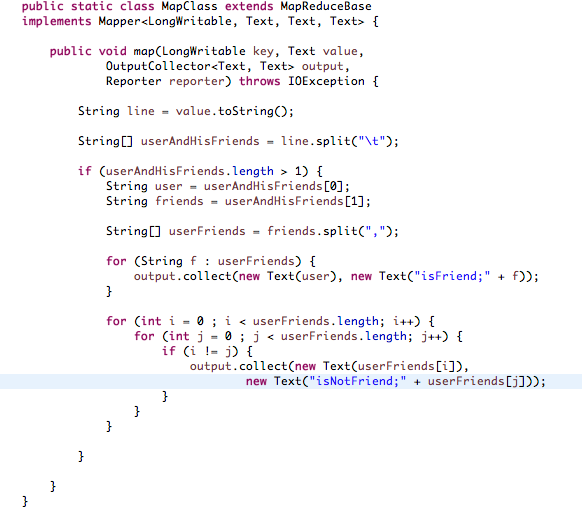
\includegraphics[width=0.5\textwidth]{plots/map.png}
	\caption{\label{mapProgram} Map method of the program resolving our problem}
\end{figure}

Figure \ref{mapProgram} provides the map method created to resolve the problem.

\begin{center}
\begin{table}
\begin{center}
\begin{tabular}{|l|l|l|l|l|}
  \hline
  Key & Value \\
  \hline
 B & isNotFriend, C \\
 B & isNotFriend, C \\
 C & isNotFriend, B \\
  C & isNotFriend, B \\
 A & isNotFriend, D \\
 A & isNotFriend, D \\
  D & isNotFriend, A \\
  \hline
\end{tabular}
\caption{\label{ReduceExampleProblem} Example results of the reduce step.}
\end{center}
\end{table}
\end{center}

\begin{center}
\begin{table}
\begin{center}
\begin{tabular}{|l|l|l|l|l|}
  \hline
  Key & Value \\
  \hline
 B & C \\
 C &  B \\
 A &  D \\
  D & A \\
  \hline
\end{tabular}
\caption{\label{ReduceExampleResults} Example results of the problem algorithm.}
\end{center}
\end{table}
\end{center}

In the reduce part, the input of the reduce method contains all the values related to a key, hence, we selected all the maps where their values contain isNotFriend and there are no couple of the same two people where the value contains isFriend. Hence, we computed and sorted all the occurrences selected. As an example, we got the results provided in Table \ref{ReduceExampleProblem}, we compute the number of occurrences to get the results provided in Table \ref{ReduceExampleResults}.



\begin{figure}
	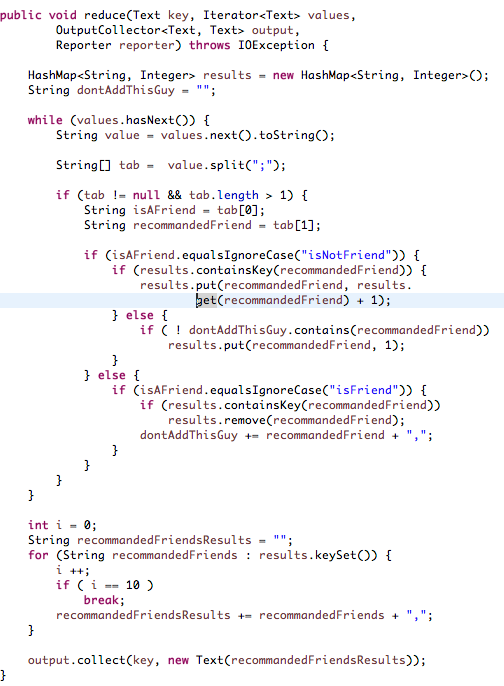
\includegraphics[width=0.5\textwidth]{plots/reduce.png}
	\caption{\label{reduceProgram} Reduce method of the program resolving our problem}
\end{figure}


Figure \ref{reduceProgram} provides the reduce method created to resolve the problem.

\begin{figure}
	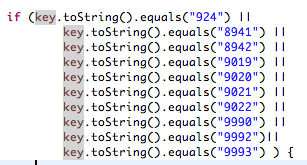
\includegraphics[width=0.4\textwidth]{plots/condition.png}
	\caption{\label{conditionProgram} Condition added to get only few results to verify the program correctness}
\end{figure}


In order to show only a part of our results, which consists of providing the recommendations of connections for the users with the following user IDs: 924, 8941, 8942, 9019, 9020, 9021, 9022, 9990, 9992, and 9993, we putted all the statements of the reduce method into a condition block, where the condition presented in Figure \ref{conditionProgram}.

\subsubsection{Results}

\begin{figure}
	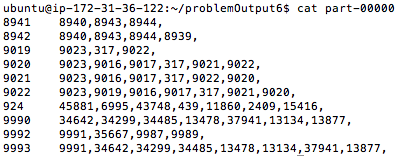
\includegraphics[width=0.5\textwidth]{plots/resultProblem.png}
	\caption{\label{resultProblem} Results of the problem in data tests (User IDs : 942, 8941, 8942, 9019, 9020, 9021, 9022, 9990, 9992, and 9993 }
\end{figure}

Figure \ref{resultProblem} provides the results of the friends recommendations problem, the program recommends to the user ID 8941, the users 8940, 8943, and 8944. It also recommends to the user ID 8942, the users 8940, 8943, 8944, and 8939.


\subsubsection{Discussion}
We conclude that MapReduce can resolve such problem that requires a navigation in network, because we can process data in multiple instances, where we can dispatch data into sub elements referred by a key (User Id in this case), and where each instance process data having the same key. Moreover, because we can dispatch data, and there is no node needing information from another node. Moreover, this problem can be divided in sub problems. Hence, MapReduce is one of the best solution for such kind of problems. 



\section{Conclusion}
\label{sec:conclusion}

By the growth of data size across time that needs to be processed, we got big data, which can be processed in many hosts at the same time, Hadoop is one of the most important frameworks enabling big data processing. We conducted in this study four experiments and we resolved a networking problem, to show when Hadoop MapReduce provides results in less time than Linux Command, and in which situations Hadoop MapReduce can be useful. We found that Linux command provides results in less time when Hadoop is configured in Pseudo distributed mode. However, Hadoop gives results in less time than Linux command when the data size is higher than 29120 bytes. We also found that time is correlated to data size in the two steps of MapReduce, reducing data size of one step (Reduce step in experiment four) can reduce the execution time. Moreover, we found that MapReduce is a solution to problems that can be divided to sub problems, and if we can't divide the execution problem, like Fibonacci series that we can't divide on sub problems, MapReduce can't be a solution.

\balance
\bibliographystyle{IEEEtran}
\bibliography{assignment.bib}


\end{document}
